\documentclass[11pt,a4paper]{article}
\usepackage[margin=1in]{geometry}
\usepackage{amsmath}
\usepackage{booktabs}
\usepackage{tikz}
\usepackage[colorlinks=true,linkcolor=blue,urlcolor=blue]{hyperref}

\title{Technical Writing with LaTeX\\\large A Practical Demonstration}
\author{Ananya Siju\\Department of Computer Science and Engineering\\MNIT Jaipur}
\date{October 2026}

\begin{document}
\maketitle
\begin{abstract}
This document demonstrates essential LaTeX features for the Technical Writing laboratory: document structure, text formatting, lists, equations, tables, figures, cross-references, and bibliographic references.
\end{abstract}

\tableofcontents
\newpage

\section{Introduction}
LaTeX is a \textbf{document preparation system} especially useful for academic and technical writing. It supports \textit{consistent formatting} and reproducible document generation. Visit the \href{https://www.latex-project.org/}{LaTeX Project} for more information.

\section{Document Structure}
A LaTeX file begins with a document class and optional packages. The visible content belongs between the \verb|\begin{document}| and \verb|\end{document}| commands.

\subsection{Advantages}
\begin{itemize}
  \item Consistent headings and page layout.
  \item High-quality mathematical notation.
  \item Automatic numbering and cross-references.
  \item Plain-text source compatible with Git.
\end{itemize}

\subsection{Typical Workflow}
\begin{enumerate}
  \item Write a \texttt{.tex} source file.
  \item Compile it using a LaTeX engine.
  \item Review the PDF and correct any errors.
  \item Commit the source to version control.
\end{enumerate}

\section{Mathematical Typesetting}
Inline mathematics can express $E=mc^2$. Equation~\eqref{eq:mean} shows the arithmetic mean of $n$ observations.
\begin{equation}
  \bar{x}=\frac{1}{n}\sum_{i=1}^{n}x_i
  \label{eq:mean}
\end{equation}

\section{Tables}
Table~\ref{tab:tools} summarizes several documentation tools.
\begin{table}[htbp]
  \centering
  \begin{tabular}{lll}
    \toprule
    Tool & Main purpose & Typical output \\
    \midrule
    LaTeX & Document typesetting & PDF \\
    Beamer & Presentations & PDF slides \\
    Doxygen & Code documentation & HTML or LaTeX \\
    Git & Version control & Commit history \\
    \bottomrule
  \end{tabular}
  \caption{Tools used in technical documentation}
  \label{tab:tools}
\end{table}

\section{Figures}
Figure~\ref{fig:workflow} illustrates a simple documentation workflow. It is drawn directly in TikZ and does not require an external image file.
\begin{figure}[htbp]
  \centering
  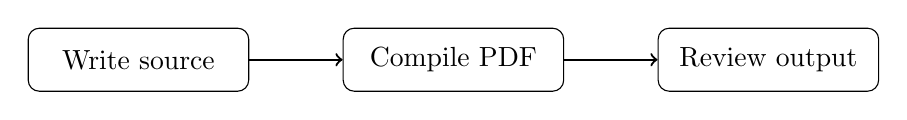
\begin{tikzpicture}[every node/.style={draw,rounded corners,minimum width=2.8cm,minimum height=0.8cm,align=center}]
    \node (a) at (0,0) {Write source};
    \node (b) at (4,0) {Compile PDF};
    \node (c) at (8,0) {Review output};
    \draw[->,thick] (a) -- (b);
    \draw[->,thick] (b) -- (c);
  \end{tikzpicture}
  \caption{Basic LaTeX documentation workflow}
  \label{fig:workflow}
\end{figure}

\section{Conclusion}
LaTeX separates document content from much of its formatting and is well suited to structured technical writing. Additional information is available from the official LaTeX documentation~\cite{latexproject}.

\begin{thebibliography}{9}
\bibitem{latexproject} The LaTeX Project, \emph{LaTeX -- A document preparation system}. \url{https://www.latex-project.org/}.
\end{thebibliography}
\end{document}
